\documentclass{beamer}

\usepackage[T2A]{fontenc}
\usepackage[utf8]{inputenc}
\usepackage[english,russian]{babel}
\usepackage{amssymb,amsfonts,amsmath,mathtext}
\usepackage{cite,enumerate,float,indentfirst}

\usepackage{graphicx}
\usepackage{booktabs}
\usepackage{tabularx}

% Attribute-Value Matrices
\usepackage{avm}
\avmfont{\sc}
\avmoptions{sorted,active}
\avmvalfont{\rm}
\avmsortfont{\scriptsize\it}

% CCG parse trees
\newcommand{\deriv}[2]
{  \renewcommand{\arraystretch}{.5}
$\begin{array}[t]{*{#1}{c}}
     #2
   \end{array}$ }
\newcommand{\gf}[1]{\textsf{\textsl{#1}}}
\newcommand{\cf}[1]{\mbox{\ensuremath{\cfont{#1}}}}
\newcommand{\uline}[1]
{\mc{#1}{\hrulefill} }
\newcommand{\mc}[2]
  {\multicolumn{#1}{c}{#2}}
\newcommand{\cfont}{\mathsf}
\newcommand{\bs}{\backslash}
\newcommand{\subsa}[1]{\hspace{-0.75mm}_{_{#1}}}
\newcommand{\subsb}[1]{\hspace{-0.10mm}_{_{#1}}}
\newcommand{\subs}[1]{\hspace{-0.40mm}_{#1}}
\newcommand{\subsf}[1]{\hspace{-0.75mm}_{_{#1}}}
\newcommand{\supsa}[1]{\hspace{-1.75mm}^{^{#1}} }
\newcommand{\supsb}[1]{\hspace{-0.80mm}^{^{#1}}  }
\newcommand{\sups}[1]{\hspace{-0.40mm}^{#1}}


\graphicspath{{images/}}

\usetheme{Pittsburgh}
\usecolortheme{whale}

\setbeamertemplate{footline}{\scriptsize{\hspace*{0.4cm}\insertframenumber}\vspace*{0.3cm}}
\beamertemplatenavigationsymbolsempty

\errorcontextlines 10000

\begin{document}
\title{\huge{SmartHouse SynSem}}
\subtitle{MMCCG \& HLDS FTW}
\author{Константин Соколов}
\institute[]
{Mathlingvo, СПбГУ, i-Free\\ \bigskip  \url{http://nlu-rg.ru}}
\date{Санкт-Петербург, 2014} 
% Создание заглавной страницы
\begin{frame}
    \thispagestyle{empty}
    \titlepage
\end{frame}

\begin{frame}{План}
    \setcounter{framenumber}{1}
    \begin{itemize}
        \item Постановка задачи
        \item Концепция решения
        \item Теоретические основы и технологии
        \item Демонстрация
        \item Результаты прототипирования, оценки
    \end{itemize}
\end{frame}


\begin{frame}{}
\begin{center}
\textbf{Большая задача}\\
\bigskip
Мультимодальное управление умным домом
\end{center}
\bigskip
\begin{center}
\textbf{Подзадача}\\
\bigskip
Семантический анализ запросов \\в рамках естественно-языкового интерфейса \\управления умным домом
\end{center}
\end{frame}

\begin{frame}{Постановка задачи}
\begin{itemize}
  \item Умный дом
	\begin{itemize}
  		\item согласованное взаимодействие разнородного оборудования
		\item обратная связь, видимость, прозрачность
		\item персонализированное, адаптивное, проактивное поведение
	\end{itemize}
  \bigskip
  \item Мультимодальное управление
	\begin{itemize}
  		\item сосуществование различных способов управления
		\item естественно-языковой интерфейс не должен уметь всё
	\end{itemize}
\end{itemize}
\end{frame}

\begin{frame}{}
\begin{center}
	\textbf{Допущения и предпосылки}\\
\end{center}
\end{frame}

\begin{frame}{Допущения и предпосылки (1)}
Командный режим работы:\\
\bigskip
\begin{itemize}
	\item Это не диалоговая система и не IVR
	\item Обратная связь
		\begin{itemize}
			\item изменение состояния устройств 
			\item панель управления
			\item носимые устройства 
			\item звуковые сигналы и пр.
		\end{itemize}
	\item Голосовое взаимодействие одностороннее
		\begin{itemize}
			\item уточнений и наводящих вопросов от системы нет
			\item синтеза речи нет
			\item \textit{mixed initiative} нет
		\end{itemize}
\end{itemize}
\end{frame}

\begin{frame}{Допущения и предпосылки (2)}
Контролируемый язык:\\
\bigskip
\begin{itemize}
	\item Две крайности, которых хотелось бы избежать:
		\begin{itemize}
			\item всё что угодно 
			\item список команд для заучивания
		\end{itemize}
	\item Ограниченный домен
		\begin{itemize}
			\item мы работаем с очень узкой предметной областью
			\item мы контролируем набор языковых конструкций и словарь
		\end{itemize}
	\item Цель: говорить как угодно, но ''только про лампочки''.
\end{itemize}
\end{frame}

\begin{frame}{Допущения и предпосылки (3)}
Дискурс:\\
\bigskip
\begin{itemize}
	\item Поддержка контекста взаимодействия в пределах сессии 
	\item В пределах сессии пользователь может
		\begin{itemize}
			\item чего-то не уточнять, предполагать известным
			\item ссылаться на предшествующее состояние системы
			\item ссылаться на свои прошлые слова
		\end{itemize}
\end{itemize}
\end{frame}

\begin{frame}{Допущения и предпосылки (4)}
Голосовое управление:\\
\bigskip
\begin{itemize}
	\item ASR может ошибаться
	\item ASR может возвращать список гипотез
	\item ASR можно настраивать с учетом текущего контекста
\end{itemize}
\end{frame}

\begin{frame}{Допущения и предпосылки (5)}
Ежедневное использование:\\
\bigskip
\begin{itemize}
	\item Пользователей мало, но они взаимодействуют постоянно
	\item Доля успешных взаимодействий должна быть большой
	\item Требуется качественный анализ и быстродействие
\end{itemize}
\end{frame}

\begin{frame}{Допущения и предпосылки (6)}
Технические особенности:\\
\bigskip
\begin{itemize}
	\item Возможность опереться на знания о системе и пользователях
	\item Возможность использовать специализированное оборудование для решения задачи управления
	\item Возможность использовать вычислительно тяжелые подходы
	\item Нет возможности ''ходить в облако''
\end{itemize}
\end{frame}

\begin{frame}{}
\begin{center}
	\textbf{Близкие области исследований}\\
\end{center}
\end{frame}

\begin{frame}{Близкие области исследований (1)}
\begin{itemize}
	\item Вычислительная семантика
		\begin{itemize}
			\item теоретико-модельная формальная семантика
			\item синтактико-семантический интерфейс
			\item NLU как компонент систем распознавания речи
		\end{itemize}
	\bigskip
	\item Искусственный интеллект
		\begin{itemize}
			\item символьные методы в компьютерной лингвистике
			\item робототехника (анализ сцен, восприятие)
			\item представление знаний и \textit{interactive grounding}
		\end{itemize}
	\bigskip
	\item Computer Science
		\begin{itemize}
			\item логический вывод
			\item проверка и построение моделей
			\item верификация программ
		\end{itemize}
\end{itemize}
\end{frame}

\begin{frame}{Близкие области исследований (2)}
\begin{itemize}
	\item Известные решения
		\begin{itemize}
			\item C\&C Tools
			\item OpenCCG
			\item LKB, PATR-II и др.
		\end{itemize}
	\bigskip
	\item Дорожки
		\begin{itemize}
			\item Recognizing Textual Entailment (c 2005 г.)
			\item Supervised Semantic Parsing of Robotic Spatial Commands (SemEval-2014)
		\end{itemize}
\end{itemize}
\end{frame}

\begin{frame}{}
\begin{center}
	\textbf{Основные проблемы}\\
\end{center}
\end{frame}


\begin{frame}{Основные проблемы (1)}
\begin{itemize}
	\item Ошибки распознавания
	\bigskip
		\begin{itemize}
			\item \texttt{``включи''} и \texttt{``выключи''}
			\item \texttt{``включи свет и лампу''} и \texttt{``включи свет у лампы''}
		\end{itemize}
		\bigskip
	\item Неоднозначность
	\bigskip
		\begin{itemize}
			\item \texttt{``красная и белая лампа''}
				\begin{itemize}
					\item две лампы, одна красная и одна белая
					\item одна красно-белая лампа (``большой и сильный человек'')
				\end{itemize}
			\item \texttt{``красная лампа в прихожей''}
				\begin{itemize}
					\item в прихожей много ламп, одна из них красная
					\item красных ламп много, одна из них в прихожей
				\end{itemize}
			\item \texttt{``включи свет и телевизор на кухне''}
				\begin{itemize}
					\item и свет, и телевизор - на кухне
					\item телевизор на кухне, свет - нет
				\end{itemize}
		\end{itemize}
\end{itemize}
\end{frame}

\begin{frame}{Основные проблемы (2)}
\begin{itemize}
	\item Учет семантических и прагматических факторов
	\bigskip
		\begin{itemize}
			\item \texttt{``включи лампу на кухне и телевизор в комнате''}
				\begin{itemize}
					\item кухня не может стоять в комнате
				\end{itemize}
			\item \texttt{``включи лампу на столе и телевизор в комнате''}
				\begin{itemize}
					\item лампа на столе, стол в комнате
					\item лампа на столе, но стол не в комнате
				\end{itemize}
			\item \texttt{``включи лампу''}
				\begin{itemize}
					\item зависимость от местоположения
					\item зависимость от конфигурации (несколько ламп)
				\end{itemize}
			\item \texttt{``сделай музыку погромче''}
				\begin{itemize}
					\item разное поведение днем и ночью
					\item различные пользовательские предпочтения
				\end{itemize}
		\end{itemize}
\end{itemize}
\end{frame}

\begin{frame}{}
\begin{center}
	\textbf{Предлагаемый подход}\\
\end{center}
\end{frame}

\begin{frame}{Предлагаемый подход (1)}
\begin{itemize}
	\item Синтактико-семантический компонент
		\begin{itemize}
			\item получает список вариантов от ASR
			\item формирует варианты интерпретации
			\item устраняет заведомо некорректные варианты
			\item расширяет пространство гипотез, делая допущения
			\item вычисляет оценки правдоподобности гипотез
			\item формирует ранжированный список гипотез
		\end{itemize}
		\bigskip
	\item Модуль принятия решений делает выбор на основе 
		\begin{itemize}
			\item прагматической информации
				\begin{itemize}
					\item местоположения пользователя
					\item состояния оборудования
					\item времени суток
				\end{itemize}
			\item эвристик и правила (интеллектуальное поведение)
			\item модели пользователя (персонализация) 
			\item статистики прошлых запросов (адаптация)
			\item текущих предпочтений (режим работы, энергосбережение)
		\end{itemize}
\end{itemize}
\end{frame}

\begin{frame}{Предлагаемый подход (2)}
Суть подхода - генерация гипотез и фильтрация\\
\bigskip
\bigskip
\resizebox{1.0\linewidth}{!}{ % Resize table to fit within \linewidth horizontally
    \begin{tabularx}{1.7\textwidth}{lcX}
    \toprule
    \textbf{Компонент}          & \textbf{Число гипотез}  & \textbf{Параметры для расчета оценки}\\
    \midrule
    Распознавание речи          & 10             & score, confidence\\ 
    Расширение запроса          & 100            & количество вставок, удалений, пропусков, словарных замен,\newline 
    											   расстояние редактирования\\ 
    Парсер                      & 100            & сложность разборов, проективность, использование доп. правил \\ 
    Логическая форма            & 200            & глубина для рекурсивных структур, количество переменных,\newline
    											   число клауз и пр.\\ 
    Оценка модели               & 10             & выполнимость всей формы или отдельных её частей\\
    \bottomrule
    \end{tabularx}
}
\end{frame}


\begin{frame}{}
\begin{center}
	\textbf{Цели}\\
\end{center}
\end{frame}


\begin{frame}{Цели прототипирования (1)}
\begin{itemize}
	\item Работа с русским языком
	\item Работа с неоднозначностью
	\item Оценка реализуемости и трудоемкости
	\item Оценка возможностей имеющихся open-source решений для работы с deep semantic parsing
	\item Оценка возможности интеграции в существующую инфраструктуру (включая интеграцию с ASR)
	\item Оценка вариативности языковых конструкций, поддающихся реализации
\end{itemize}
\end{frame}

\begin{frame}{Цели прототипирования (2)}
НЕ ставились цели:\\
\bigskip
\begin{itemize}
	\item Достичь быстродействия системы или оценить его
	\item Покрытие кейсов по сценариям использования системы конечным пользователем
\end{itemize}
\end{frame}

\begin{frame}{Цели демонстрации (1)}
\begin{itemize}
	\item Рассказать о теоретических основах подхода
	\item Рассказать об используемых компонентах
	\item Рассказать об используемых формализмах
	\item Посмотреть на реализацию разборов \\конкретных типов предложений
	\item Дать оценки по исходным задачам прототипа
\end{itemize}
\end{frame}

\begin{frame}{Цели демонстрации (2)}
\begin{itemize}
	\item Рассказать об ограничених текущего прототипа и как их можно решать
	\item Рассказать, что еще не было сделано
	\item Рассказать о дополнительных возможностях, которые может предостаавить выбранный подход
\end{itemize}
\end{frame}


\begin{frame}{}
\begin{center}
	\textbf{Теоретический минимум и технологии}\\
\end{center}
\end{frame}


\begin{frame}{Теоретический минимум}
\begin{itemize}
	\item Multimodal Combinatory Categorial Grammar (MMCCG)
	\item Hybrid Logic Dependency Semantics (HLDS)
	\item Hybrid Logic Model Checking (HLMC)
\end{itemize}
\end{frame}

\begin{frame}{MMCCG}
\begin{center}
\texttt{This page intentionally left blank}
\end{center}
\end{frame}

\begin{frame}{Модальная логика}
Модальный оператор $\Box$\\
\bigskip
\begin{itemize}
	\item $\Box \phi$ - ``необходимо p''
	\item $\Diamond \phi$ - ``возможно p''
	\item $\Diamond \phi \; \equiv \; \sim \Box \sim \phi$
\end{itemize}
\bigskip
Аксиомы некоторых модальных систем:
\begin{itemize}
  \item \textbf{K: } $\Box (\phi \supset \psi) \supset ( \Box \phi \supset \Box \psi)$
  \item \textbf{T: } $\Box \phi \supset \phi$
  \item \textbf{S4:} $\Box \phi \supset \Box \Box \phi$
\end{itemize}
\bigskip
\end{frame}

\begin{frame}{Реляционная семантика (1)}
\textit{Шкала Крипке} (Kripke frame):\\
\bigskip
$\mathcal{F} = (W, R)$, где $W$ - непустое множество, $R \subseteq W \times W$.\\
\bigskip
\begin{itemize}
  \item $w_i \in W$ - миры, состояния, точки отнесенности
  \item $R$ - отношение достижимости
  \item если $wRv$, то говорят, что $v$ \textit{возможен относительно} $w$
\end{itemize}
\end{frame}

\begin{frame}{Реляционная семантика (2)}
\textit{Модель Крипке} $\mathcal{M} = (\mathcal{F}, V)$, где  
\bigskip
\begin{itemize}
  \item $\mathcal{F}$ - шкала Крипке
  \item $V : P \to 2^W$ - функция оценивания, т.е. отображение из атомарных выражений в подмножества множества миров
\end{itemize}
\bigskip
\end{frame}

\begin{frame}{Реляционная семантика (3)}
Пусть $\mathcal{M} = (\mathcal{F}, V)$, $w \in W$, $\phi$ - формула, $p \in P$\\
\bigskip
Истинность $\phi$ в модели $\mathcal{M}$ в точке $w$ определяется рекурсивно\\
\bigskip
\begin{itemize}
  \item $\mathcal{M}, w \models p \; \Longleftrightarrow \; w \in V(p)$
  \item $\mathcal{M}, w \models \neg \phi \; \Longleftrightarrow \; \mathcal{M}, w \not\models \phi$
  \item $\mathcal{M}, w \models \phi \vee \psi \; \Longleftrightarrow \; \mathcal{M}, w \models \phi$ или $\mathcal{M}, w \models \psi$
  \item $\mathcal{M}, w \models \Box \phi \; \Longleftrightarrow \; \forall v \in W \; . \; (w R v \to \mathcal{M}, v \models \phi)$
  \item $\mathcal{M}, w \not\models \perp$
\end{itemize}
\bigskip
Если $\mathcal{M}, w \models \phi$, говорят, что $\phi$ \textit{логически следует} из $\mathcal{M}, w$
\end{frame}

\begin{frame}{Мультимодальная логика}
\begin{itemize}
	\item Набор модальных операторов $\Box_i$ (соотв., $\Diamond_i$)
	\item Шкала Крипке - размеченный граф
\end{itemize}
\end{frame}

\begin{frame}{Гибридная логика (1)}
\begin{itemize}
	\item Будем писать $\langle \pi \rangle$ и $[\pi]$ вместо $\Diamond_\pi$ и $\Box_\pi$
	\item $\langle \pi \rangle \alpha \; \equiv \; \neg [\pi] \neg \alpha$
	\item Введем дополнительно класс \textit{номиналов} (обозн. $i, j, k$)
	\item Введем оператор $@_i$ со значением ``истинно в точке $i$''
\end{itemize}
\bigskip
Язык гибридной логики $HL(@)$:\\
\begin{center}
$WFF_{HL(@)} := \top \; \vert \; i \; \vert \; p \; \vert \; \neg \alpha \; | \; \alpha \wedge \beta \; \vert \; \langle \pi \rangle \alpha \; \vert \; @_i \alpha$
\end{center}
\end{frame}

\begin{frame}{Гибридная логика (2)}
Гибридная модель Крипке:\\
\bigskip
\begin{center}
$\mathcal{M} = (W, \{R_\pi \vert \pi \in MOD\}, V)$, где\\
\bigskip
\begin{itemize}
	\item $\mathcal{F} = (W, \{R_\pi \vert \pi \in MOD\})$ - шкала Крипке
	\item $V : PROP \cup NOM \to 2^W$
	\item $V(i)$ - синглетон
\end{itemize}
\end{center}
\end{frame}

\begin{frame}{Гибридная логика (3)}
Денотационная семантика для $HL(@)$:\\
\bigskip
\begin{itemize}
	\item $\mathcal{M}, w \models i \; \Leftrightarrow \; w = V(i)$
	\item $\mathcal{M}, w \models @_i \alpha \; \Leftrightarrow \; \mathcal{M}, w' \models \alpha$ и $w' = V(i)$
\end{itemize}
\end{frame}

\begin{frame}[fragile]
\frametitle{Гибридная логика и XML (1)}
{\footnotesize 
\begin{verbatim}
<biblio>
    <book id="b1">
        <author>Marx</author>
        <author>de Rijke</author>
        <title>Hybrid Logics</title>
        <date>1998</date>
        <cites idref="b1"/>
    </book>
    <book id="b2">
        <author>Franceschet</author>
        <title>Model Checking</title>
        <date>2000</date>
        <cites idref="a1"/>
    </book>
</biblio>
\end{verbatim}
}
\end{frame}

\begin{frame}{Гибридная логика и XML (2)}
XML документ - модель, формула гибридной логики - запрос.\\
\bigskip
\begin{itemize}
\item Существует ли в точности одна книга автора Franceschet?
	\begin{itemize}
		{\scriptsize \item $@_{root} \langle biblio \rangle \langle book \rangle \downarrow x \; . \; \langle author \rangle Franceschet \; \wedge \; @_{root} \langle biblio \rangle [book] x$}
	\end{itemize}
\bigskip	
\item Существует ли две разных книги?	
	\begin{itemize}
		{\scriptsize \item $@_{root} \langle biblio \rangle \langle book \rangle \downarrow x \; . \; @_{root} \langle biblio \rangle \langle book \rangle \neg x$}
	\end{itemize}
\end{itemize}
\end{frame}

\begin{frame}{Гибридная логика и проверка моделей}
Дана гибридная модель $\mathcal{M}$ и формула $\alpha$, найти все узлы в $\mathcal{M}$, в которых $\alpha$ истинна:
\bigskip
\begin{center}
    $T(\mathcal{M}, \alpha) = \{ w \in W \; | \; \mathcal{M}, w \models \alpha \}$
\end{center}
\end{frame}

\begin{frame}{Hybrid Logic Dependency Semantics}
Hybrid Logic Dependency Semantics:\\
\bigskip
\begin{itemize}
	\item Композициональный семантический формализм 
	\item Описание семантических структур зависимостей с помощью выражений гибридной логики
	\item Cемантическая композиция реализуется как унификация логических форм (ср. с формализмами на основе $\lambda$-исчисления: конкатенация с последующей редукцией)
	\item Реализован в системе OpenCCG (Baldridge et al., 2007)
\end{itemize}
\end{frame}

\begin{frame}{Технологии}
\begin{itemize}
	\item OpenCCG (Baldridge et al., 2007)
	\item Грамматика Moloko (DFKI)
	\item HLMC (L. Dragone)
\end{itemize}
\end{frame}

\begin{frame}{}
\begin{center}
	\textbf{Формализмы}\\
\end{center}
\end{frame}


\begin{frame}{dotCCG (1)}
\begin{itemize}
	\item DSL для создания MMCCG-грамматик
	\item Транслируется в XML-формат OpenCCG
	\item MOLOKO - около 4 kLOC 
	\item Мой прототип - около 0.5 kLOC (из-за морфологии)
\end{itemize}
\end{frame}

\begin{frame}[fragile]
\frametitle{dotCCG (2)}
Определение семейства слов:
{\footnotesize \begin{verbatim}
family tv(V) {
    entry : s \! np / np : 	E:event(* <Actor>(S:entity) 
                                      <Patient>(X:entity));
}
\end{verbatim}}
\bigskip
\bigskip
Запись в словарной части:
{\footnotesize \begin{verbatim}
word лампа:Noun(thing, pred=лампа) {
    лампа:  s-sg nom fem;
    лампу:  s-sg acc fem;
    лампы:  s-pl nom fem;
    лампы:  s-pl acc fem;
}
\end{verbatim}}
\end{frame}

\begin{frame}[fragile]
\frametitle{dotCCG (3)}
Правила изменения типа:
{\footnotesize \begin{verbatim}
rule {
    typechange: s<10> [E NUM PERS MOOD POL FIN VFORM vf-to-imp] \! 
                np<9> [S nom NUM PERS nf-real] / 
                np<2> [X acc]
             => s<~10>[E fin-full s-imp] / 
                np<2> [X acc] : E:event(<Mood>(imp) 
                                        <Subject>(S:entity 
                                                 addressee));
}
\end{verbatim}}
\end{frame}

\begin{frame}[fragile]
\frametitle{dotCCG (4)}
Фрагмент онтологии:
{\footnotesize \begin{verbatim}
feature {
    ont-event: event { 
                   action 
               };

    ont-entity: entity {
                     physical {
                            animate { person },
                            thing,
                            e-location { e-region, e-place }
  		             }
  		        };
};  		        
\end{verbatim}}
\end{frame}

\begin{frame}[fragile]
\frametitle{dotCCG (5)}
Макросы:
{\footnotesize \begin{verbatim}
def COORD(args)       { R( args <First>(F) ^ <Next>(N) ) }

# Адъективное склонение, твердая разновидность
def adj-adj-h-sg-fem(base) {
    # sg, fem
    base."ая" : nom s-sg s-degree-base fem pre-n;
    base."ой" : gen s-sg s-degree-base fem pre-n;
    base."ой" : dat s-sg s-degree-base fem pre-n;
    base."ую" : acc s-sg s-degree-base fem pre-n;
    base."ой" : abl s-sg s-degree-base fem pre-n;
    base."ой" : loc s-sg s-degree-base fem pre-n;
}
\end{verbatim}}
\end{frame}

\begin{frame}[fragile]
\frametitle{HLDS (1)}
Компактная форма:
{\footnotesize \begin{verbatim}
@w0:action(ON ^
           <Mood>imp ^
           <Actor>x1:entity ^
           <Patient>(w2:thing ^ лампа ^
                     <Num>sg ^
                     <Modifier>(w1:q-color ^ красный-adj) ^
                     <Modifier>(w3:m-location ^ на ^
                                <Anchor>(w4:e-place ^ кухня ^
                                         <Num>sg))))
\end{verbatim}}
\end{frame}

\begin{frame}[fragile]
\frametitle{HLDS (2)}
Линеаризованная форма:
{\footnotesize \begin{verbatim}
@E_0:action(CLOSE) ^ 
@E_0:action(<Mood>imp) ^
@E_0:action(<Actor>S_0:entity) ^ 
@E_0:action(<Patient>T_1:thing) ^ 
@M_3:m-location(в) ^ 
@M_3:m-location(<Anchor>T_4:e-place) ^ 
@T_1:thing(шторы) ^ 
@T_1:thing(<Num>pl) ^ 
@T_1:thing(<Modifier>M_3:m-location) ^ 
@T_4:e-place(прихожая) ^ 
@T_4:e-place(<Num>sg))
\end{verbatim}}
\end{frame}

\begin{frame}[fragile]
\frametitle{HLDS (3)}
HLDS в виде AVM:\\
\begin{center}
	\begin{avm}
	[{action} predicate & on \cr
    	      Mood & imp \cr 
        	  Actor & @{1} \cr 
	          Patient & [{thing} predicate & @{2} лампа \cr
    	                         Num & sg \cr 
        	                     Modifier & [{q-color} predicate & красный\_adj ]]]
	\end{avm}
\end{center}	
\end{frame}

\begin{frame}[fragile]
\frametitle{HLMC (1)}
Выражение на языке гибридной логики для HLMC:
{\footnotesize \begin{verbatim}
# без номиналов
shtory & <num>(pl) & <modifier>(na & <anchor>(kuhnya & <num>(sg)))

# с номиналами и переменными
@root (B x (<thing>(x <modifier>(<anchor>(kuhnya)))))
\end{verbatim}}
\end{frame}

\begin{frame}[fragile]
\frametitle{HLMC (2)}
Гибридная модель Крипке для HLMC (описывается в XML).
\begin{center}
	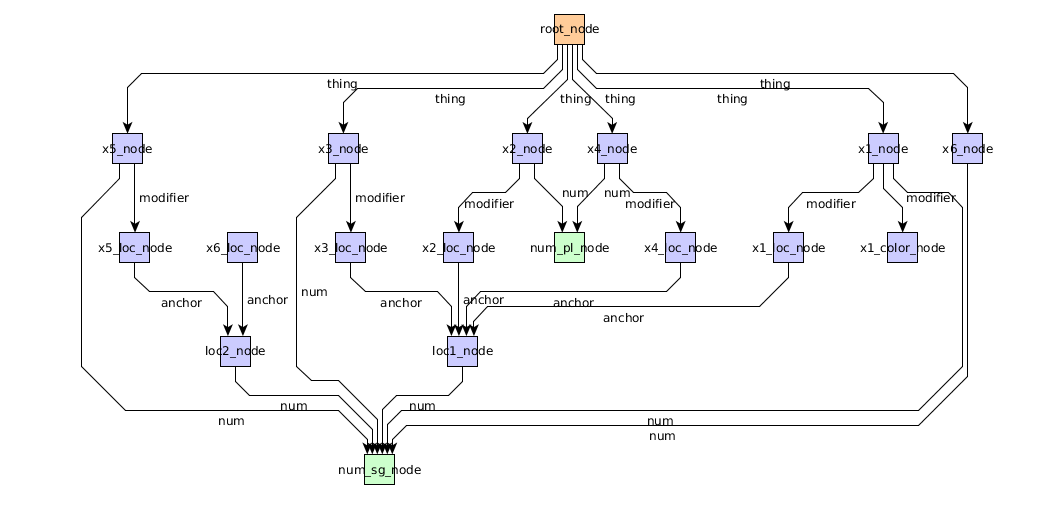
\includegraphics[scale=0.3]{model.png}
\end{center}
\end{frame}


\begin{frame}{}
\begin{center}
	\textbf{Пример анализа}
\end{center}
\end{frame}

\begin{frame}{Пример анализа (1)}
\begin{center}
\texttt{включи лампу и подсветку на кухне
}\end{center}
\end{frame}

\begin{frame}{Пример анализа (2)}
Первый вариант разбора (MMCCG):\\
\bigskip
\begin{center}
\deriv{6}{
\gf{включи} & \gf{лампу} & \gf{и} & \gf{подсветку} & \gf{на} & \gf{кухне} \\
\uline{1} & \uline{1} & \uline{1} & \uline{1} & \uline{1} & \uline{1} \\
\cf{s\bs \supsa{-} np/ np} & \cf{np} & \cf{n/ np\bs \subsb{*} np} & \cf{n} & \cf{pp/ \subsa{\diamond} np} & \cf{np} \\
& \mc{2} {\hrulefill_{<}} \\
& \mc{2}{\cf{n/ np}} \\
&&&& \mc{2} {\hrulefill_{>}} \\
&&&& \mc{2}{\cf{pp}} \\
&&&& \mc{2} {\hrulefill_{t\mathbf{ypechange-6}}}\\
&&&& \mc{2}{\cf{n\bs \subsb{*} n}} \\
&&& \mc{3} {\hrulefill_{<}} \\
&&& \mc{3}{\cf{n}} \\
&&& \mc{3} {\hrulefill_{t\mathbf{ypechange-3}}}\\
&&& \mc{3}{\cf{np}} \\
& \mc{5} {\hrulefill_{>}} \\
& \mc{5}{\cf{n}} \\
& \mc{5} {\hrulefill_{t\mathbf{ypechange-4}}}\\
& \mc{5}{\cf{np}} \\
 \mc{6} {\hrulefill_{>}} \\
 \mc{6}{\cf{s\bs \supsa{-} np}} \\
}
\end{center}
\end{frame}

\begin{frame}[fragile]
\frametitle{Пример анализа (3)}
Первый вариант разбора (HLDS):\\
\bigskip
\begin{center}
{\scriptsize \begin{verbatim}
@w0:action(ON ^ 
              <Mood>imp ^ 
              <Actor>x1:entity ^ 
              <Patient>(w2:entity ^ и ^ 
                        <Num>pl ^ 
                        <First>(w1:thing ^ лампа ^ 
                                <Num>sg) ^ 
                        <Next>(w3:thing ^ подсветка ^ 
                               <Num>sg ^ 
                               <Modifier>(w4:m-location ^ на ^ 
                                          <Anchor>(w5:e-place ^ кухня ^ 
                                                   <Num>sg))) ^ 
                        <Num>pl))
\end{verbatim}
}                        
\end{center}
\end{frame}

\begin{frame}[fragile]
\frametitle{Пример анализа (4)}
Первый вариант разбора (HLMC):\\
\bigskip
\begin{center}
{\scriptsize \begin{verbatim}
>   ON (lampa & <num>(sg)) : x1_node x6_node 

>   ON (podsvetka & <num>(sg) & 
        <modifier>((na & <anchor>((kuhnya & <num>(sg)))))) : x3_node 
\end{verbatim}
}                        
\end{center}
\end{frame}

\begin{frame}{Пример анализа (5)}
Второй вариант разбора (MMCCG):\\
\bigskip
\begin{center}
\deriv{6}{
\gf{включи} & \gf{лампу} & \gf{и} & \gf{подсветку} & \gf{на} & \gf{кухне} \\
\uline{1} & \uline{1} & \uline{1} & \uline{1} & \uline{1} & \uline{1} \\
\cf{s\bs \supsa{-} np/ np} & \cf{np} & \cf{n/ np\bs \subsb{*} np} & \cf{np} & \cf{pp/ \subsa{\diamond} np} & \cf{np} \\
& \mc{2} {\hrulefill_{<}} \\
& \mc{2}{\cf{n/ np}} \\
&&&& \mc{2} {\hrulefill_{>}} \\
&&&& \mc{2}{\cf{pp}} \\
& \mc{3} {\hrulefill_{>}} \\
& \mc{3}{\cf{n}} \\
&&&& \mc{2} {\hrulefill_{t\mathbf{ypechange-6}}}\\
&&&& \mc{2}{\cf{n\bs \subsb{*} n}} \\
& \mc{5} {\hrulefill_{<}} \\
& \mc{5}{\cf{n}} \\
& \mc{5} {\hrulefill_{t\mathbf{ypechange-4}}}\\
& \mc{5}{\cf{np}} \\
 \mc{6} {\hrulefill_{>}} \\
 \mc{6}{\cf{s\bs \supsa{-} np}} \\
}
\end{center}
\end{frame}

\begin{frame}[fragile]
\frametitle{Пример анализа (6)}
Второй вариант разбора (HLDS):\\
\bigskip
\begin{center}
{\scriptsize \begin{verbatim}
@w0:action(ON ^ 
              <Mood>imp ^ 
              <Actor>x1:entity ^ 
              <Patient>(w2:entity ^ и ^ 
                        <Num>pl ^ 
                        <First>(w1:thing ^ лампа ^ 
                                <Num>sg) ^ 
                        <Modifier>(w4:m-location ^ на ^ 
                                   <Anchor>(w5:e-place ^ кухня ^ 
                                            <Num>sg)) ^ 
                        <Next>(w3:thing ^ подсветка ^ 
                               <Num>sg) ^ 
                        <Num>pl))
\end{verbatim}
}                        
\end{center}
\end{frame}

\begin{frame}[fragile]
\frametitle{Пример анализа (7)}
Второй вариант разбора (HLMC):\\
\bigskip
\begin{center}
{\scriptsize \begin{verbatim}
>   ON (lampa & <num>(sg) & 
        <modifier>((na & <anchor>((kuhnya & <num>(sg)))))) : x1_node 

>   ON (podsvetka & <num>(sg) & 
        <modifier>((na & <anchor>((kuhnya & <num>(sg)))))) : x3_node 
\end{verbatim}
}                        
\end{center}
\end{frame}

\begin{frame}{Другие примеры (1)}
\begin{itemize}
	\item лампа
	\item красная лампа
	\item включи красную лампу
	\item выключи красную лампу
	\item включи красную лампу на кухне
	\item включи лампу на кухне
	\item включи красную лампу и подсветку
\end{itemize}
\end{frame}

\begin{frame}{Другие примеры (2)}
\begin{itemize}
	\item включи красную лампу на кухне и подсветку
	\item включи красную лампу и подсветку на кухне
	\item включи лампу на кухне и подсветку в прихожей
	\item включи лампу и выключи подсветку
	\item включи красную лампу и выключи лампу на кухне
	\item включи красную лампу и закрой шторы на кухне
\end{itemize}
\end{frame}

\begin{frame}{Другие примеры (3)}
\begin{itemize}
	\item включи и выключи лампу
	\item включи и выключи лампу на кухне
	\item включи и выключи лампу и подсветку на кухне
	\item включи лампу и лампочку и подсветку на кухне 
	\item включи и выключи лампу на кухне и подсветку в прихожей
	\item включи и выключи лампу на столе и подсветку в прихожей
\end{itemize}
\end{frame}


\begin{frame}{}
\begin{center}
	\textbf{Выводы и оценки}
\end{center}
\end{frame}

\begin{frame}{Работа с русским языком}
\begin{itemize}
	\item Простые типы предложений портируются легко
	\item Необходимо аккуратно реализовать онтологию
	\item Трудоемкая реализация морфологии (но ср.: RusForIR)
	\item Программировать не нужно
	\item Работа для лингвиста (или нескольких)
	\item Отличные возможности для повторного использования
	\item Реализация большого фрагмента русского языка в формализме MMCCG 
может стать существенным вкладом в отечественную компьютерную лингвистику
\end{itemize}
\end{frame}

\begin{frame}{Работа с неоднозначностью}
\begin{itemize}
	\item Удалось реализовать все предполагавшиеся варианты
	\item ... и обнаружить еще несколько
\end{itemize}
\end{frame}

\begin{frame}{Что предстоит сделать}
\begin{itemize}
	\item Поддержка дискурса
	\item Расчет оценок
	\item Портирование HLMC и поддержка типов
	\item Автоматизация создания модели
\end{itemize}
\end{frame}

\begin{frame}{Оценка трудоемкости}
\begin{itemize}
	\item Грамматика - около месяца
	\item Model Checking - до двух недель
	\item Модуль принятия решений - не удалось оценить
\end{itemize}
\end{frame}

\begin{frame}{Новые возможности}
\begin{itemize}
	\item Генерация правого контекста для распознавания речи
	\item Валидация модели
	\item Извлечение семантических ролей
\end{itemize}
\end{frame}

\begin{frame}{}
    \thispagestyle{empty}
    \begin{center}
        {\large Спасибо!}
    \end{center}
\end{frame}


%%% слайд помещается сюда
%% \begin{frame}{Заголовок}
%% \end{frame}

\end{document}
